\documentclass[aspectratio=169,10pt]{beamer}

% =====================================================================
%  ENIGMA — AI Academy DLE-AI-202 Final Presentation
%  Early Warning of Hydrate Formation in Offshore Well Service Lines
%  Compile: pdflatex slides.tex  (run TWICE)
% =====================================================================

\usetheme{Madrid}
\usecolortheme{seahorse}
\usefonttheme{professionalfonts}

% Packages
\usepackage[utf8]{inputenc}
\usepackage[T1]{fontenc}
\usepackage{amsmath,amssymb}
\usepackage{graphicx}
\usepackage{booktabs}
\usepackage{url}
\usepackage{xcolor}
\usepackage{multirow}

% Figure path: works both on Overleaf (figures/) and locally (../figures/)
\graphicspath{{figures/}{../figures/}}

% Remove navigation dots
\setbeamertemplate{navigation symbols}{}

% Footer
\setbeamertemplate{footline}{
  \leavevmode%
  \hbox{%
  \begin{beamercolorbox}[wd=.4\paperwidth,ht=2.25ex,dp=1ex,center]{author in head/foot}%
    \usebeamerfont{author in head/foot}Team Enigma \(\cdot\) AI Academy 2026
  \end{beamercolorbox}%
  \begin{beamercolorbox}[wd=.4\paperwidth,ht=2.25ex,dp=1ex,center]{title in head/foot}%
    \usebeamerfont{title in head/foot}\insertshorttitle
  \end{beamercolorbox}%
  \begin{beamercolorbox}[wd=.2\paperwidth,ht=2.25ex,dp=1ex,right]{date in head/foot}%
    \usebeamerfont{date in head/foot}\insertframenumber{} / \inserttotalframenumber\hspace*{2em}
  \end{beamercolorbox}}%
  \vskip0pt%
}

% ---- Title info ----
\title[Hydrate Early Warning]{Early Warning of Hydrate Formation\\in Offshore Well Service Lines}
\subtitle[XGBoost vs. TCN vs. GRU at Matched FAR]{XGBoost vs. TCN vs. GRU at Matched False-Alarm Budgets\\
3W Dataset 2.0.0 -- Event 9}
\author[Team Enigma]{
  Mammadova,~Aisel \and Huseynov,~Shamistan \and Karimova,~Rahima\\
  Mammadova,~Gulnur \and Arabova,~Saida
}
\institute[AI Academy]{AI Academy, Baku, Azerbaijan\\
DLE-AI-202, Cohort I 2026 \(\cdot\) Track 2}
\date{September 2026}

% =====================================================================
\begin{document}
% =====================================================================

\begin{frame}[plain]
  \titlepage
\end{frame}

% ---- Outline ----
\begin{frame}{Outline}
  \tableofcontents
\end{frame}

% =====================================================================
\section{Motivation \& Problem}
% =====================================================================

\begin{frame}{Why Does This Matter?}
  \begin{columns}
    \column{0.55\textwidth}
      \begin{block}{The Hazard}
        Gas hydrates crystallize inside subsea service lines at high pressure \& low temperature.
        \begin{itemize}
          \item Complete blockage $\Rightarrow$ well shutdown
          \item Costly interventions, safety risk
          \item Loss of production for days to weeks
        \end{itemize}
      \end{block}
      \begin{block}{The Opportunity}
        The \textbf{transient phase} is detectable before blockage.\\
        An alarm at transient onset gives operators lead time to:
        \begin{itemize}
          \item Inject methanol / glycol inhibitor
          \item Reduce backpressure
          \item Warm the line
        \end{itemize}
      \end{block}
    \column{0.43\textwidth}
      \begin{alertblock}{Research Question}
        Can a deep learning model detect the transient onset \textbf{earlier} than a feature-engineered baseline, at a \textbf{controlled false-alarm rate}?
      \end{alertblock}
      \vspace{0.5em}
      \textbf{Headline metric:} Lead time (minutes from first alarm to annotated transient onset) at a target FAR of $\leq 1$ alarm per 100 operating hours.
  \end{columns}
\end{frame}

% =====================================================================
\section{Dataset}
% =====================================================================

\begin{frame}{3W Dataset 2.0.0 — Event 9}
  \begin{columns}
    \column{0.48\textwidth}
      \textbf{Instance counts}
      \begin{table}
        \begin{tabular}{lr}
          \toprule
          Split & Count \\
          \midrule
          Real instances (Event 9) & 57 \\
          \quad w/ Transient phase & \textbf{14} \\
          \quad reaching blockage & 3 \\
          Simulated instances & 150 \\
          Normal-operation & 594 \\
          \bottomrule
        \end{tabular}
      \end{table}
      \vspace{0.4em}
      \begin{alertblock}{Critical Fact}
        Only \textbf{14} real transient events across \textbf{7 wells}.\\
        This is the hardest constraint in the project.
      \end{alertblock}
    \column{0.50\textwidth}
      \textbf{Key dataset properties}
      \begin{itemize}
        \item Severity is \textbf{monotonic}: Normal $\to$ Transient $\to$ Established. Verified in all 57 instances.
        \item Missingness in \textit{every} real instance (median 11.2\%, max 50.4\%)
        \item 3 instances: sensors dead for entire recording
        \item Hydrate wells $\cap$ Normal wells $= \emptyset$\\(15 vs. 9 wells, completely disjoint)
        \item Per-instance normalization is \textbf{mandatory} (not cosmetic)
      \end{itemize}
      \vspace{0.4em}
      \textbf{Preprocessing:} 1\,Hz $\to$ 1/30\,Hz (decimation), 60-sample windows = 30\,min, stride 150\,s, 5-channel subset.
  \end{columns}
\end{frame}

\begin{frame}{Annotated Sensor Trace}
  \begin{center}
    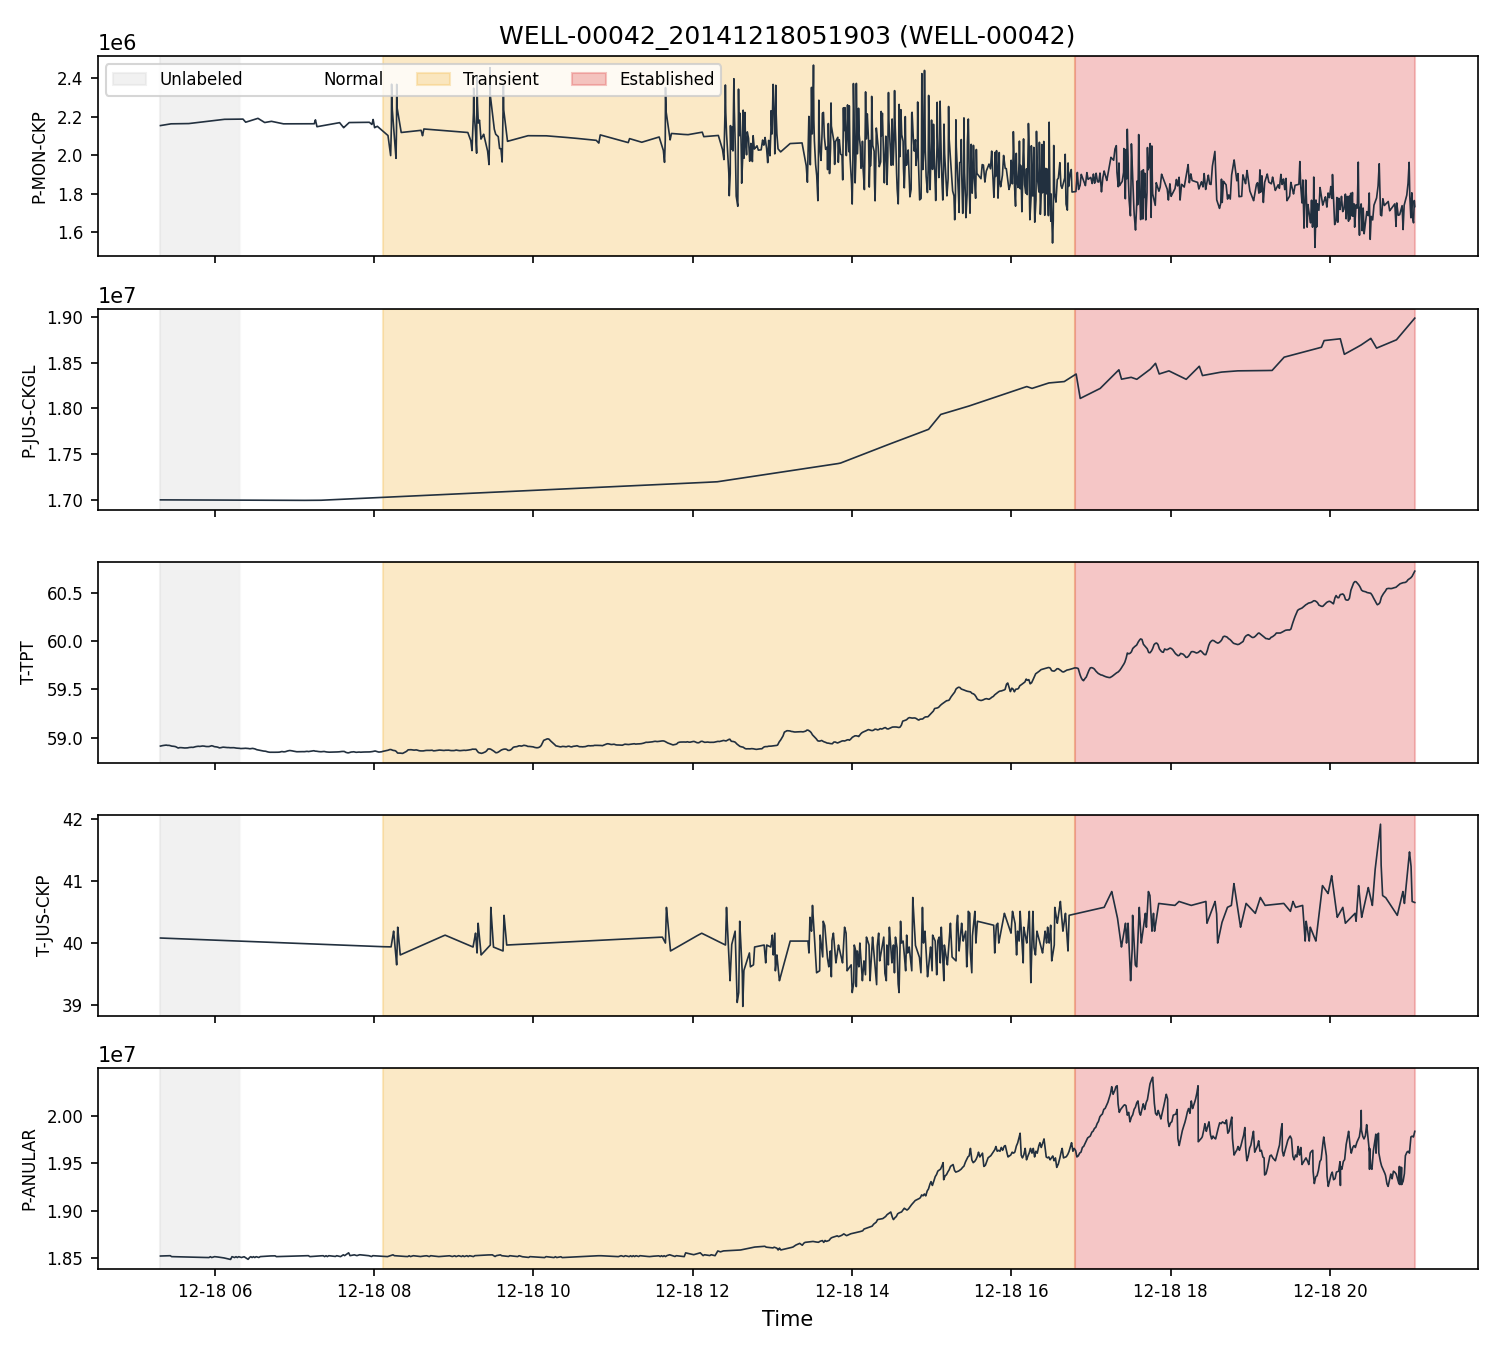
\includegraphics[width=0.88\textwidth,height=0.62\textheight,keepaspectratio]{annotated_trace.png}
  \end{center}
  \vspace{-0.5em}
  \small Colour bands: \textcolor{green!60!black}{Normal} / \textcolor{orange!80!black}{Transient} / \textcolor{red}{Established}. Lead time measured from first alarm (dashed line) to Transient onset.
\end{frame}

% =====================================================================
\section{Method}
% =====================================================================

\begin{frame}{Feature Engineering — XGBoost Baseline}
  \begin{block}{Multi-timescale, mask-aware features (95 total)}
    For each of 5 channels, extract 3 causal slices (full / last-half / last-quarter) $\times$ 6 stats (mean, std, min, max, slope, net-change) $\Rightarrow$ 90 features.\\
    Plus: per-channel \textbf{presence fraction} (5 features) — fraction of non-missing samples.
  \end{block}
  \begin{columns}
    \column{0.55\textwidth}
      \textbf{Why presence fraction matters:}
      \begin{itemize}
        \item 40.8\% of XGBoost gain concentrated on 5 presence columns
        \item Presence-only model achieves 74\% of full performance \textit{with no sensor values at all}
        \item Root cause: sensor availability is well-specific \& acts as a proxy for well identity
      \end{itemize}
    \column{0.43\textwidth}
      \begin{alertblock}{Important caveat}
        The baseline partly reads \textbf{instrumentation} patterns, not physical hydrate dynamics.\\
        Feature importance does not reproduce across folds ($\tau$ = +0.20, +0.40, $-$0.40).
      \end{alertblock}
  \end{columns}
\end{frame}

\begin{frame}{Deep Model Architectures}
  \begin{columns}
    \column{0.48\textwidth}
      \begin{block}{TCN — Temporal Convolutional Network}
        \begin{itemize}
          \item 4 temporal blocks, kernel $k=3$
          \item Dilations: $\{1, 2, 4, 8\}$
          \item Receptive field: \textbf{61 samples} $>$ window size 60
          \item Causal convolutions (no future look-ahead)
          \item Mask concatenated at input
          \item 3-class softmax output
        \end{itemize}
      \end{block}
    \column{0.48\textwidth}
      \begin{block}{GRU — Gated Recurrent Unit}
        \begin{itemize}
          \item Single-layer \textbf{unidirectional} GRU
          \item Hidden size: 64
          \item Mask concatenated at each timestep
          \item 3-class linear readout
          \item Unidirectional = causal by construction
        \end{itemize}
      \end{block}
  \end{columns}
  \vspace{0.5em}
  Both models: class-weighted cross-entropy, early stopping on validation PR-AUC (patience=10), best checkpoint saved, trained on A100 GPU with AMP.
\end{frame}

% =====================================================================
\section{Experimental Setup}
% =====================================================================

\begin{frame}{Cross-Validation Design — Preventing Leakage}
  \begin{columns}
    \column{0.52\textwidth}
      \begin{block}{Why standard CV fails here}
        Hydrate wells and Normal wells are \textbf{disjoint populations}.\\
        A single \texttt{StratifiedGroupKFold} cannot balance both simultaneously.
      \end{block}
      \textbf{Solution: two independent grouped splits}
      \begin{enumerate}
        \item Split 7 positive-event wells by well ID
        \item Split 9 normal wells balanced by operating hours
        \item Pair splits to form 3 complete folds
      \end{enumerate}
      \begin{alertblock}{Simulation policy}
        Simulated instances: \textbf{training only}. Never in validation or test.
      \end{alertblock}
    \column{0.46\textwidth}
      \textbf{Fold composition}
      \begin{table}
        \begin{tabular}{cccc}
          \toprule
          Fold & Val.~pos. & Test~pos. & Test hrs \\
          \midrule
          0 & 1 & 5 & 509h \\
          1 & 3 & 5 & 557h \\
          2 & 5 & 4 & 531h \\
          \bottomrule
        \end{tabular}
      \end{table}
      \vspace{0.4em}
      \small Fold 0: \textbf{only 1} positive validation event — threshold selection is unreliable. This is a structural dataset constraint (7 wells, 3 folds), not a bug.
  \end{columns}
\end{frame}

\begin{frame}{Evaluation Protocol — S3 Freeze}
  \begin{enumerate}
    \item \textbf{Train}: fit model on training fold (weights frozen after)
    \item \textbf{Validate}: sweep 200 thresholds on \textit{validation} Normal instances,\\
          select highest threshold where FAR $\leq 1\%$/h
    \item \textbf{Test}: apply frozen threshold to \textit{test} fold — \textbf{no further changes}
  \end{enumerate}
  \vspace{0.5em}
  \begin{columns}
    \column{0.48\textwidth}
      \begin{block}{Alarm definition}
        Smoothed probability (causal trailing mean) above threshold for $\geq$ \texttt{min\_duration} seconds = one alarm onset.\\
        \textbf{Centered smoothing = test leakage.} Guarded by \texttt{test\_alarm.py}.
      \end{block}
    \column{0.48\textwidth}
      \begin{block}{Three headline metrics}
        \begin{itemize}
          \item \textbf{Event recall}: fraction of events with an alarm before transient onset
          \item \textbf{Lead time}: $t_{\text{transient}} - t_{\text{first alarm}}$ (minutes)
          \item \textbf{FAR}: alarm onsets / normal hours
        \end{itemize}
      \end{block}
  \end{columns}
\end{frame}

% =====================================================================
\section{Results}
% =====================================================================

\begin{frame}{XGBoost Baseline — Validation PR-AUC}
  \begin{columns}
    \column{0.52\textwidth}
      \begin{table}
        \caption{Validation PR-AUC (positive base rate 3.34\%)}
        \begin{tabular}{cccc}
          \toprule
          Fold & Pos.~val.~events & real\_only & real+sim \\
          \midrule
          0 & 1 & 0.0005 & 0.0003 \\
          1 & 3 & \textbf{0.7755} & 0.2420 \\
          2 & 5 & 0.0751 & 0.1288 \\
          \midrule
          \multicolumn{2}{c}{mean $\pm$ sd} & $0.28 \pm 0.43$ & $0.12 \pm 0.12$ \\
          \bottomrule
        \end{tabular}
      \end{table}
    \column{0.46\textwidth}
      \begin{alertblock}{PR-AUC is not comparable across folds}
        Fold 0: 1 positive window in 11,260 (base rate $10^{-4}$)\\
        Fold 1: 463 positive in 7,327 (base rate 6.3\%)\\
        PR-AUC rises mechanically with the base rate.\\
        Fold variance = \textbf{47$\times$} feature-design variance.
      \end{alertblock}
  \end{columns}
  \vspace{0.4em}
  \textbf{Simulated data did not help XGBoost.} Paired difference real+sim $-$ real\_only = $-0.16 \pm 0.33$ (negative in 2 of 3 folds).
\end{frame}

\begin{frame}{Head-to-Head: Event Recall}
  \begin{columns}
    \column{0.5\textwidth}
      \begin{table}
        \caption{Event Recall at matched FAR ($\leq 1\%$/h)}
        \begin{tabular}{lcc}
          \toprule
          Model & real\_only & real+sim \\
          \midrule
          \textbf{XGBoost} & $\mathbf{0.233 \pm 0.252}$ & $0.167 \pm 0.289$ \\
          TCN & $0.083 \pm 0.144$ & $0.000 \pm 0.000$ \\
          GRU & $0.000 \pm 0.000$ & $0.067 \pm 0.115$ \\
          \bottomrule
        \end{tabular}
      \end{table}
      \vspace{0.3em}
      \begin{table}
        \caption{Mean Lead Time (minutes, detected events only)}
        \begin{tabular}{lcc}
          \toprule
          Model & real\_only & real+sim \\
          \midrule
          \textbf{XGBoost} & $\mathbf{43.4}$ & 209.9 \\
          TCN & 89.3 & --- \\
          GRU & --- & 34.9 \\
          \bottomrule
        \end{tabular}
      \end{table}
    \column{0.48\textwidth}
      \begin{exampleblock}{Key takeaway}
        XGBoost (real\_only) is the \textbf{only model} with consistent non-zero recall across multiple folds.\\[0.5em]
        Deep models detected events in 1 fold only (out of 3), making their lead-time numbers unreliable single observations.\\[0.5em]
        \textbf{Simulated data hurt every model} on the headline metric (real test distribution).
      \end{exampleblock}
  \end{columns}
\end{frame}

\begin{frame}{Lead Time vs. False Alarm Rate Trade-off}
  \begin{center}
    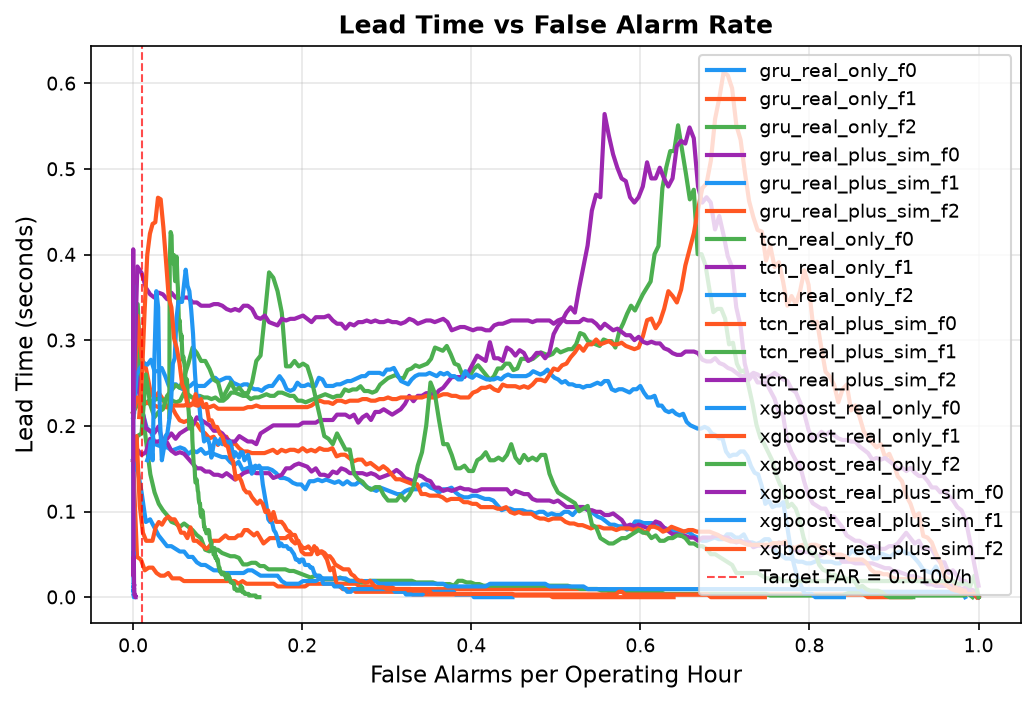
\includegraphics[width=0.68\textwidth,height=0.46\textheight,keepaspectratio]{lead_time_vs_far.png}
  \end{center}
  \small Vertical dashed line = target operating point (1 alarm / 100 h). XGBoost (real\_only) is the only model that consistently achieves non-zero lead time at or near the target FAR.
\end{frame}

\begin{frame}{The Budget, Not the Ranking, Costs the Recall}
  \begin{columns}
    \column{0.46\textwidth}
      \begin{table}
        \caption{Best achievable XGBoost event recall vs.\ false-alarm budget}
        \begin{tabular}{lcccc}
          \toprule
          alarms/h & 0.01 & 0.10 & 0.25 & 0.50 \\
          \midrule
          real\_only & 0.167 & 0.317 & \textbf{0.917} & 0.917 \\
          real+sim   & 0.167 & 0.450 & \textbf{0.917} & 0.917 \\
          \bottomrule
        \end{tabular}
      \end{table}
    \column{0.5\textwidth}
      \begin{alertblock}{Threshold tuning is not the problem}
        Re-selecting the threshold \textit{on the test fold itself} --- an oracle we could never ship --- changes recall in \textbf{0 of 6} XGBoost cells.
      \end{alertblock}
      \begin{exampleblock}{Why 1 alarm/100\,h is so severe}
        A test fold has 523--855 Normal hours, so the budget permits only \textbf{5--9 false alarms across $\approx$120 Normal recordings}. The 4--5 event recordings must rank in the top few percent of \textit{all} recordings.
      \end{exampleblock}
  \end{columns}
  \vspace{0.3em}
  \small Relaxing to 1 alarm/4\,h moves recall $0.167 \rightarrow \mathbf{0.917}$: a deployment trade-off, not a defect.
\end{frame}

\begin{frame}{Per-Well Lead Time Distribution}
  \begin{center}
    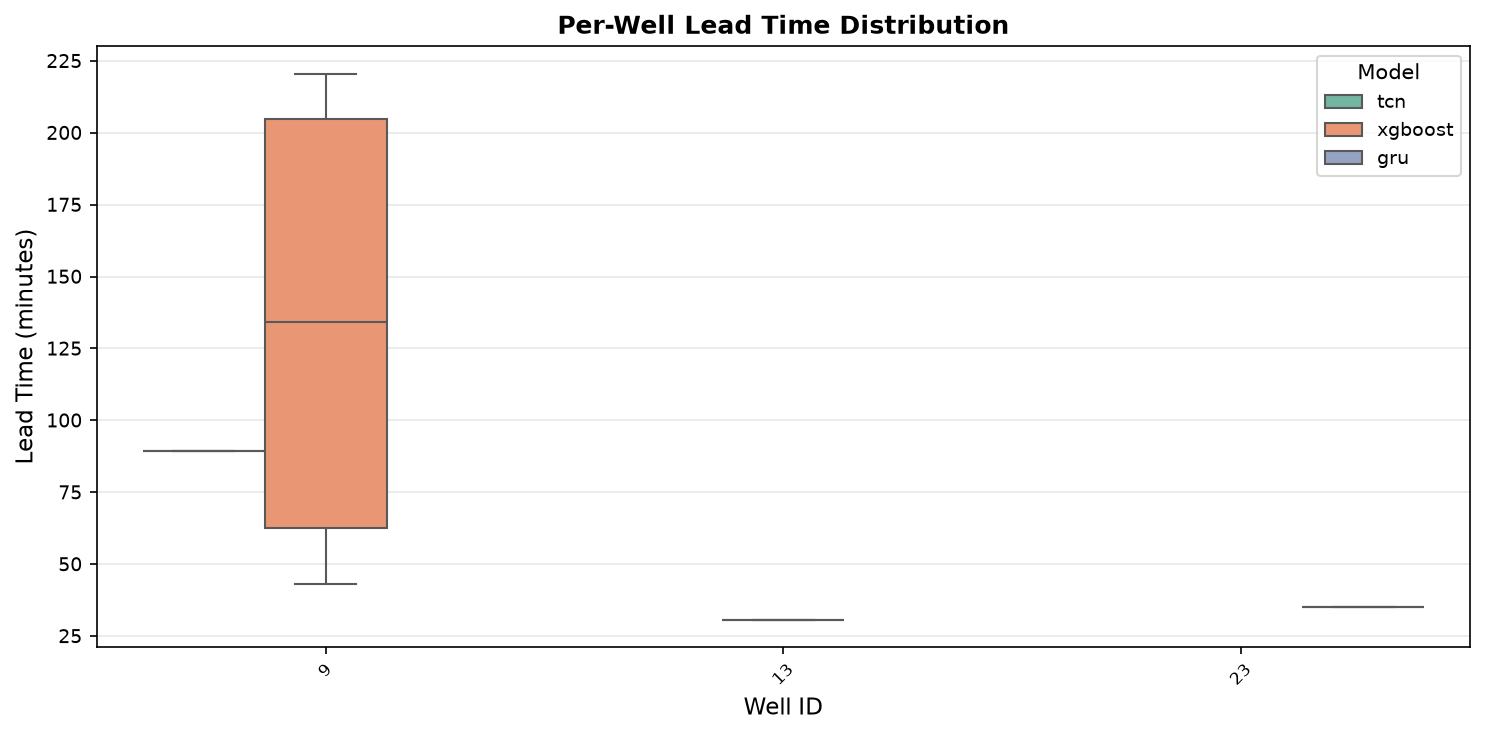
\includegraphics[width=0.75\textwidth,height=0.62\textheight,keepaspectratio]{per_well_lead_time.png}
  \end{center}
  \small High inter-well variability reflects different sensor configurations and noise profiles. With only 7 wells, no single number is representative.
\end{frame}

\begin{frame}{XGBoost Calibration}
  \begin{columns}
    \column{0.55\textwidth}
      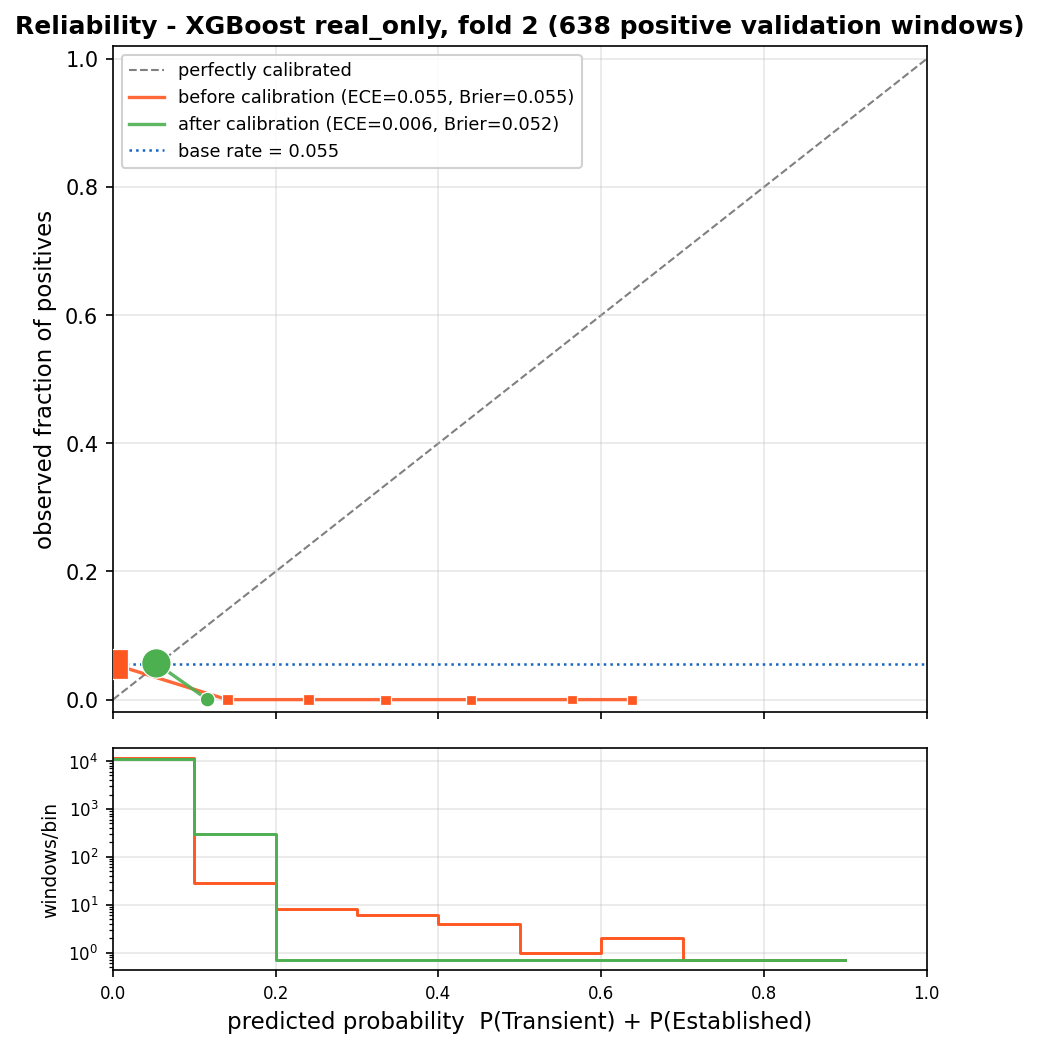
\includegraphics[width=\textwidth,height=0.70\textheight,keepaspectratio]{reliability_xgboost.png}
    \column{0.43\textwidth}
      \begin{block}{Platt scaling results}
        \begin{itemize}
          \item ECE: $0.041 \to 0.008$ (real\_only)\\
                $0.054 \to 0.011$ (real+sim)
          \item Brier score: $-29\%$ in all 6 cells
          \item Improvement consistent across all folds and conditions
        \end{itemize}
      \end{block}
      \begin{block}{Why it matters}
        Threshold selection sweeps the probability axis. Without calibration the threshold doesn't transfer from validation to test.
      \end{block}
  \end{columns}
\end{frame}

% =====================================================================
\section{Discussion}
% =====================================================================

\begin{frame}{Why Deep Models Underperformed}
  \begin{columns}
    \column{0.50\textwidth}
      \begin{alertblock}{14 events is simply not enough}
        Gradient-based models with thousands of parameters need dozens of positive events to learn transition dynamics.\\
        With 14 events across 3 folds, fold~0's single validation event makes threshold selection equivalent to random.
      \end{alertblock}
      \begin{block}{What we would do next time}
        \begin{enumerate}
          \item SSL pretraining on 594 normal instances
          \item Then fine-tune on labeled events
          \item Expected: better representations without more labeled data
        \end{enumerate}
      \end{block}
    \column{0.48\textwidth}
      \begin{block}{Why sim data hurt}
        \begin{itemize}
          \item Simulated: \textbf{90.3\%} positive windows
          \item Real: \textbf{3.34\%} positive windows
          \item Factor of $\approx$27 distributional mismatch
          \item Model trains on a ``hydrate-certain'' world, tested on a ``hydrate-rare'' world
          \item Threshold calibration breaks
        \end{itemize}
      \end{block}
      \begin{block}{Sensor shortcut}
        XGBoost's 40.8\% gain on presence-fraction columns = reading which well has which sensors, not hydrate physics.\\
        Important caveat on generalizability.
      \end{block}
  \end{columns}
\end{frame}

% =====================================================================
\section{Conclusion}
% =====================================================================

\begin{frame}{Conclusion \& Recommendations}
  \begin{block}{Summary}
    \begin{itemize}
      \item XGBoost (real\_only): best recall \textbf{23.3\%}, lead time \textbf{43.4\,min}, FAR \textbf{7.9\%/h} --- no fold met the 1\%/h budget on test (2.6$\times$, 19$\times$, 2.0$\times$ over)
      \item TCN: 8.3\% recall (1 fold only), lead time 89.3\,min — promising but unreliable
      \item GRU: 0\% recall under real\_only — did not generalize
      \item Simulated data: consistently hurts all models on real test wells
    \end{itemize}
  \end{block}
  \begin{columns}
    \column{0.5\textwidth}
      \begin{exampleblock}{Recommendation for operators}
        Deploy XGBoost (real\_only), but \textbf{choose the alarm budget deliberately}. At 1 alarm/100\,h it recalls 17\%; at 1 alarm/4\,h the same model recalls \textbf{92\%}. The events are detectable --- the pre-registered tolerance is what excludes them.
      \end{exampleblock}
    \column{0.48\textwidth}
      \begin{block}{Future directions}
        \begin{enumerate}
          \item Acquire more labeled real Event-9 data
          \item SSL pretraining on normal-operation archives
          \item Multi-well domain adaptation
          \item Physics-informed regularization
        \end{enumerate}
      \end{block}
  \end{columns}
  \vspace{0.4em}
  \small Code \& data: \url{https://github.com/AMammedova/team-hydrate3w} (tag \texttt{v1.0-final})
\end{frame}

% =====================================================================
\section*{Contributions}
% =====================================================================

\begin{frame}{Team Enigma — Contributions}
  \begin{table}
    \footnotesize
    \begin{tabular}{p{3.5cm} p{8.2cm}}
      \toprule
      \textbf{Member} & \textbf{Contributions (Code, Report, \& Slides)} \\
      \midrule
      Mammadova, Aisel (M1) & Data analysis, annotated trace, Sec.~I \& III, Slides 1--3 \\
      \addlinespace[3pt]
      Huseynov, Shamistan (M2) & Grouped CV design, fold report, Sec.~V, Slide 4 \\
      \addlinespace[3pt]
      Karimova, Rahima (M3) & 95-feature extractor, XGBoost tuning \& ablation, Sec.~IV-A \& VI-A, Slide 5 \\
      \addlinespace[3pt]
      Mammadova, Gulnur (M4) & TCN \& GRU architectures, A100 GPU training, Sec.~II \& VI-B, Slides 6--7 \\
      \addlinespace[3pt]
      Arabova, Saida (M5) & Eval pipeline, alarm logic, \texttt{run\_all.sh}, Abstract, Sec.~IV-C, VI-C, VII, VIII, Slides 8--14 \\
      \bottomrule
    \end{tabular}
  \end{table}
\end{frame}

\begin{frame}{Acknowledgements \& Tools}
  \begin{itemize}
    \item \textbf{Dataset:} Petrobras 3W Dataset 2.0.0 (Vargas et al., 2019)
    \item \textbf{Compute:} AI Academy A100 GPU (80\,GB VRAM)
    \item \textbf{Libraries:} Python 3.x, PyTorch 2.3.1, XGBoost 2.0.3, scikit-learn 1.5.0, NumPy, Pandas, Matplotlib
    \item \textbf{AI assistance:} Large Language Models were used to help structure evaluation boilerplate code, format \LaTeX{} tables, and draft documentation. All AI-generated content was reviewed, tested, and validated by the team.
  \end{itemize}
  \vspace{1em}
  \begin{center}
    \Large \textbf{Thank you. Questions welcome.}\\[0.5em]
    \normalsize \url{https://github.com/AMammedova/team-hydrate3w}
  \end{center}
\end{frame}

\end{document}
